\section{Aufbau der Testumgebung}

\begin{figure}[htbp]
    \centering
      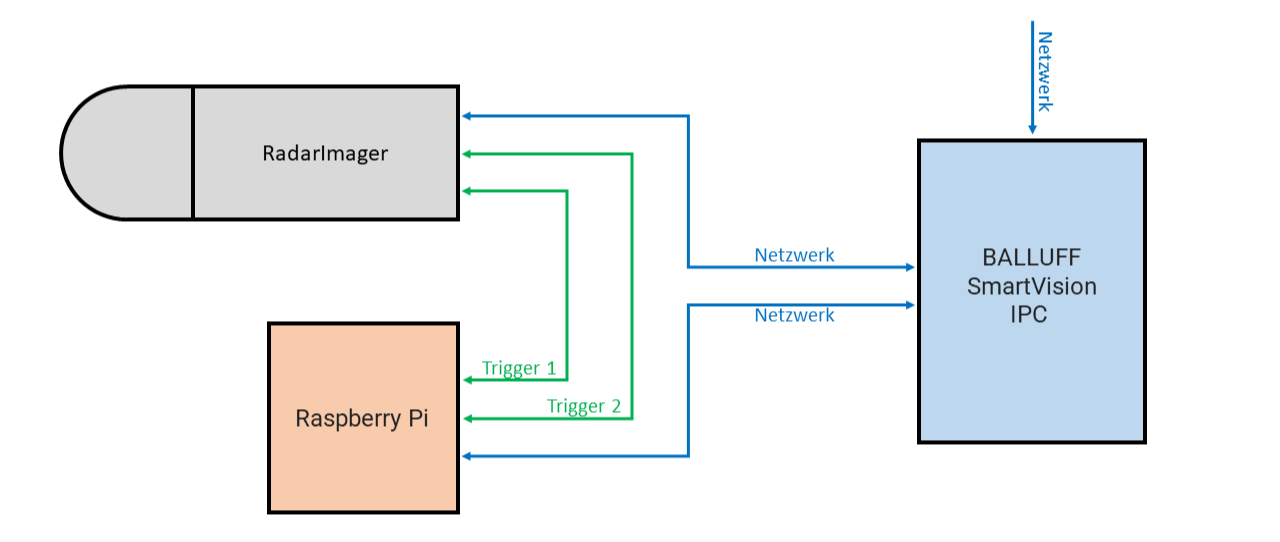
\includegraphics [width=0.9\textwidth]{Testumgebung.png}
    \caption[Testumgebung]{Testumgebung (eigene Darstellung)}
    \label{fig:Testumgebung}
\end{figure}

Abbildung \ref{fig:Testumgebung} zeigt den schematischen Aufbau der Testumgebung. Der RadarImager ist über ein Netzwerk mit einem \ac{IPC} verbunden, auf dem Ubuntu als 
Linux-Distribution läuft. Zusätzlich ist der IPC über ein weiteres Netzwerk mit einem Raspberry Pi verbunden, der einen Hardware-Trigger simuliert. Somit wird kein komplexer 
Aufbau mit Lichtschranken und einem Förderband benötigt, um Triggersignale zu erzeugen. Das Intervall und der Abstand zwischen den einzelnen Signalen ist 
einstellbar. Bei Implementierungen werden die Trigger durch externe Mechanismen wie beispielsweise eine Lichtschranke oder durch eine individuelle Lösung des Kunden erzeugt.
Die Ansteuerung des Raspberry Pi erfolgt über eine REST-API vom IPC aus. Eine REST-API (Representational State Transfer Application Programming Interface) ist eine 
Programmierschnittstelle, die den Datenaustausch zwischen verschiedenen Softwareanwendungen über das Internet ermöglicht. Sie verwendet standardisierte HTTP-Methoden, um 
Ressourcen abzurufen, zu erstellen, zu bearbeiten oder zu löschen. Die Übertragung der Bilder vom RadarImager zum IPC erfolgt über das Netzwerk unter Verwendung des 
GenICam-Standards. Zum Empfangen und Verarbeiten der Bilder auf dem IPC wird der GenICam-Client verwendet. Dieser wird im Laufe dieser Arbeit für die Tests verbessert und 
weiterentwickelt. Um das Senden der Bilder bzw. Bildstapel zu simulieren, wird während der Weiterentwicklung ein NVIDIA Jetson Orin NX verwendet, welcher auch im RadarImager verbaut ist. 
Dieser sendet synthetische Bilder auf die gleiche Weise, wie der RadarImager reale Bilder sendet. Der Einsatz des NVIDIA Jetson Orin NX ermöglicht eine erhebliche Kosteneinsparung in der Entwicklungsphase, da die Kosten für dieses Gerät nur wenige hundert 
Euro betragen. Im Gegensatz dazu kostet der komplette RadarImager mit Radarmodulen und anderen Hardwarekomponenten etwa 30.000 Euro. Darüber hinaus bietet dies die Möglichkeit, vorhandene RadarImager für andere Zwecke zu nutzen, 
beispielsweise für Demonstrationen bei potenziellen Kunden.